\begin{refsection}

\chapter{Majorise-Minimise for Deep Networks}
\label{chap:nn-maj-min}

\begin{tcolorbox}
This chapter derives architectural perturbation bounds for deep linear networks. When combined with the functional majorisation of a loss function, the bounds yield novel \textit{architecture aware} optimisation methods.
\end{tcolorbox}

Chapter \ref{chap:maj-min} developed a framework for deriving optimisation algorithms for generic machine learning problems. In essence, the framework describes a majorise-minimise meta-algorithm \citep{mm} for composite optimisation problems that apply an error measure to a function projected on to data.

The present chapter specialises this framework to machine learning problems that involve deep neural networks. Again, the framework works in three steps:

\begin{enumerate}[label=Step \arabic*:, leftmargin=*, font=\sffamily]
    \item Majorise a series expansion of the loss function in perturbations to the network output projected on to the training set.
    \item Derive architectural perturbation bounds that express the sensitivity of the network output to weight perturbations. The form of these bounds depends on details such as the width and depth of the network.
    \item Substitute the architectural perturbation bounds into the majorisation of the loss and minimise to obtain an optimisation algorithm.
\end{enumerate}

\subsection{A note on related work}

\citet{cohen2021gradient} express concern that majorise-minimise style optimisation theories (or ones based on Majorisation \ref{eq:gd-major} in particular) may be too pessimistic for deep learning. On the contrary, this chapter obtains various useful architectural scaling rules for learning rate from a majorise-minimise analysis.

While the depth scaling relation presented in this chapter is an original contribution of the thesis author and collaborators \citep{my-fromage}, the width scaling relation was first derived separately via the \textit{tensor programs} framework \citep{yang2021tuning}. That framework amounts to a perturbation analysis of neural networks with random weights operating in the asymptotic limit of infinite width. The width scaling relation in this chapter resulted from discussions with Greg Yang about how to reconcile the tensor programs framework with the non-asymptotic, non-random framework presented in this thesis. The experiments in Figures \ref{fig:width-depth} and \ref{fig:width-depth-lesion} were run as part of that collaboration.

\section{The deep linear network}

This chapter deals mainly with deep networks with identity nonlinearity $\phi = \Id$.
\begin{definition}[Deep linear network]\label{def:dln}
A \textit{deep linear network} $f$ of depth $L$ maps an input $x\in\R^{d_0}$ to an output $f(x;w) \in \R^{d_L}$ via $L$ matrix multiplications:
\begin{equation}\label{eq:dln}
f(x; w) \coloneqq W_L W_{L - 1} \dots W_1 \cdot x.
\end{equation}
In this expression, $w$ denotes the tuple $w = (W_1,...,W_L)$ for $W_l\in \R^{d_l\times d_{l-1}}$.
\end{definition}
This choice of \textit{non-nonlinearity} greatly simplifies the analysis. Although architectural perturbation bounds have been obtained for more general nonlinearities \citep{my-fromage}, the results obtained for deep linear networks in this chapter were already found to transfer experimentally to deep relu networks (Figure \ref{fig:width-depth}). It is important to note that the optimisation landscape of the deep linear network is still non-convex due to the product of weight matrices.

The following definition will aid the analysis of deep linear networks:
\begin{definition}[Output scale of the deep linear network]\label{def:output-scale}
The \textit{output scale} of a deep linear network $f$ with weight matrices $w = (W_1,...,W_L)$ is given by:
\begin{equation}
F(w) \coloneqq \sqrt{d_0}\cdot\prod_{l=1}^L \norm{W_l}_*.
\end{equation}
\end{definition}

The output scale provides a simple bound on the magnitude of network outputs:
\begin{lemma}[Output bound]
\label{lem:lipschitz} For a deep linear network $f(\cdot,w)$ and all hyperspherically constrained inputs $x\in\sqrt{d_0}\cdot\Sph^{d_0-1}$, the output magnitude obeys:
\begin{equation}
    \Vert f(x; w) \Vert_2 \leq F(w).
\end{equation}
\end{lemma}
\begin{proof} Recursively extract operator norms from the matrix product:
    \begin{align*}
        \norm{f(x;w)}_2 &= \norm{W_L W_{L - 1} \dots W_1 \cdot x}_2 \\&\leq \norm{W_L}_* \cdot \norm{W_{L - 1} \dots W_1 \cdot x}_2 
        \leq ... \leq \prod_{l=1}^L \norm{W_l}_* \cdot \norm{x}_2.
    \end{align*}
    Finally, substituting $\norm{x}_2 = \sqrt{d_0}$ completes the proof.
\end{proof}

\section{Architectural perturbation bounds for deep linear networks}

The deep linear network admits the following architectural perturbation bounds:
\begin{lemma}[Architectural perturbation bounds for the deep linear network]
\label{lem:deep_perturbation_bounds} Consider perturbing the weights of a deep linear network $f:\R^{d_0}\times\mathcal{W}\to\R$ from $w=(W_1,...,W_L)\in\mathcal{W}$ to $w+\Delta w=(W_1+\Delta W_1,...,W_L+\Delta W_L)\in\mathcal{W}$. For any collection of $m$ inputs $X\in (\sqrt{d_0}\cdot\Sph^{d_0-1})^m$, the following bounds hold:
\begin{align}
    \frac{\norm{\Delta f_X}_2}{\sqrt{m}} &\leq F(w) \cdot \left[ \prod_{l = 1}^L \left( 1 + \frac{\Vert \Delta W_l \Vert_{*}}{\Vert W_l \Vert_{*}}\right)  - 1 \right];\label{eq:drt}\\
    \frac{\norm{\Delta f_X - \nabla_w f_X \Delta w}_2}{\sqrt{m}} &\leq F(w) \cdot \left[ \prod_{l = 1}^L \left( 1 + \frac{\Vert \Delta W_l \Vert_{*}}{\Vert W_l \Vert_{*}}\right)  - 1 - \sum_{l = 1}^L \frac{\Vert \Delta W_l \Vert_{*}}{\Vert W_l \Vert_{*}} \right].\label{eq:jrt}
\end{align}
\end{lemma}
These architectural perturbation bounds involve a product over the relative size of the perturbation to each network layer, reflecting the product structure of the network itself. At large depth, the bounds are roughly exponential in the layerwise perturbation size.

While the best way to understand the results is by working out a few examples (for two, three and four layer networks, say) a formal proof is now given.

\begin{proof}[Proof of Lemma \ref{lem:deep_perturbation_bounds}] The result is shown by induction over depth $L$ for a network with multiple outputs $d_L>1$ and a single input $X=\{x\}$. The result for multiple inputs $m>1$ and a single output $d_L=1$ is then immediate.

For the base case $L=1$, the relevant network to consider is given by $f(x;w) = W_1\cdot x.$ Observe that $\nabla_w f_{\{x\}} \Delta w = \Delta W_1 \cdot x$, and also:
\begin{align*}
    \Delta f_{\{x\}} &\coloneqq f(x;w+\Delta w) - f(x;w) = (W_1 + \Delta W_1)\cdot x - W_1\cdot x = \Delta W_1 \cdot x.
\end{align*}
The base case is established by noting $\norm{\Delta f_{\{x\}} - \nabla_w f_{\{x\}} \Delta w}_2=0$, and also:
\begin{align*}
\norm{\Delta f_{\{x\}}}_2 &\leq \norm{\Delta W_1}_* \cdot \norm{x}_2 = \norm{\Delta W_1}_* \cdot \sqrt{d_0}.
\end{align*}

For the inductive step, the relevant network is given by $f(x;w) = W_L\mydots W_1\cdot x$. To tackle Inequality \ref{eq:drt}, observe that:
\begin{align*}
    &\norm{\Delta f_{\{x\}}}_2 \coloneqq \norm{f(x;w+\Delta w) - f(x;w)}_2\\
    & = \norm{(W_L+\Delta W_L) \mydots (W_1+\Delta W_1)\cdot x - W_L \mydots W_1\cdot x}_2\\
    & = \|(W_L+\Delta W_l)\cdot  \left[(W_{L-1}+\Delta W_{L-1}) \mydots (W_1+\Delta W_1)\cdot x - W_{L-1} \mydots W_1\cdot x\right] \\
    & \qquad + \Delta W_L W_{L-1} \mydots W_1\cdot x \|_2 \\
    &\leq (\norm{W_L}_* + \norm{\Delta W_L}_*)\cdot\norm{(W_{L-1}+\Delta W_{L-1}) \mydots (W_1+\Delta W_1) x - W_{L-1} \mydots W_1x}_2 \\
    & \qquad + \norm{\Delta W_L}_*\cdot \norm{W_{L-1}}_* \cdot\mydots\cdot \norm{W_1}_*\cdot\sqrt{d_0},
\end{align*}
where the last line follows by several applications of the triangle inequality and the operator norm bound. Then, by the inductive hypothesis:
\begin{align*}
    &\norm{\Delta f_{\{x\}}}_2 \leq  (\norm{W_L}_* + \norm{\Delta W_L}_*) \cdot \frac{F(w)}{\norm{W_L}_*} \cdot \left[ \prod_{l=1}^{L-1} \left( 1 + \frac{\Vert \Delta W_l \Vert_{*}}{\Vert W_l \Vert_{*}}\right)  - 1 \right]\\
    &\qquad\qquad\qquad\qquad+ \norm{\Delta W_L}_* \cdot \norm{W_{L-1}}_* \cdot\mydots\cdot \norm{W_1}_*\cdot \sqrt{d_0} \\
    &\qquad= \left(1 + \frac{\norm{\Delta W_L}_*}{\norm{W_L}_*}\right) \cdot F(w) \cdot \left[ \prod_{l=1}^{L-1} \left( 1 + \frac{\Vert \Delta W_l \Vert_{*}}{\Vert W_l \Vert_{*}}\right)  - 1 \right]+ \frac{\norm{\Delta W_L}_*}{\norm{W_L}_*}\cdot F(w)\\
    &\qquad= F(w)\cdot \left[ \prod_{l=1}^{L} \left( 1 + \frac{\Vert \Delta W_l \Vert_{*}}{\Vert W_l \Vert_{*}}\right)  - 1 \right],
\end{align*}
which establishes Inequality \ref{eq:drt}. Next, to tackle Inequality \ref{eq:jrt}, observe that:
\begin{align*}
    &\norm{\Delta f_{\{x\}} - \nabla_w f_{\{x\}}\Delta w}_2 \coloneqq \norm{f(x;w+\Delta w) - f(x;w)-\nabla_w f_{\{x\}}\Delta w}_2\\
    & = \big\|(W_L+\Delta W_L) \mydots (W_1+\Delta W_1)\cdot x - W_L \mydots W_1\cdot x \\
    &\qquad - \sum_{l=1}^L W_L\mydots W_{l+1} \Delta W_l W_{l-1}\mydots W_1 \cdot x \big\|_2 \\
    & = \big\|(W_L+\Delta W_L)\cdot\big[ (W_{L-1}+\Delta W_{L-1}) \mydots (W_1+\Delta W_1)\cdot x - W_{L-1} \mydots W_1\cdot x \\
    & \qquad - \sum_{l=1}^{L-1} W_{L-1}\mydots W_{l+1} \Delta W_l W_{l-1}\mydots W_1 \cdot x \big] \\ &\qquad +\Delta W_L \sum_{l=1}^{L-1} W_{L-1}\mydots W_{l+1} \Delta W_l W_{l-1}\mydots W_1 \cdot x \big\|_2 \\
    & \leq (\norm{W_L}_*+\norm{\Delta W_L}_*)\cdot\big\|(W_{L-1}+\Delta W_{L-1}) \mydots (W_1+\Delta W_1)x - W_{L-1} \mydots W_1 x \\
    & \qquad - \sum_{l=1}^{L-1} W_{L-1}\mydots W_{l+1} \Delta W_l W_{l-1}\mydots W_1 \cdot x \big\|_2 \\ &\qquad +\norm{\Delta W_L}_* \cdot \sum_{l=1}^{L-1} \norm{W_{L-1}}_*\mydots \norm{W_{l+1}}_* \norm{\Delta W_l}_* \norm{W_{l-1}}_*\mydots \norm{W_1}_* \cdot \sqrt{d_0},
\end{align*}
where the last line follows by several applications of the triangle inequality and the operator norm bound. Then, by the inductive hypothesis:
\begin{align*}
&\norm{\Delta f_{\{x\}} - \nabla_w f_{\{x\}}\Delta w}_2\\
& \leq (\norm{W_L}_*+\norm{\Delta W_L}_*)\cdot
    \frac{F(w)}{\norm{W_L}_*} \cdot \left[ \prod_{l=1}^{L-1} \left( 1 + \frac{\Vert \Delta W_l \Vert_{*}}{\Vert W_l \Vert_{*}}\right)  - 1 - \sum_{l=1}^{L-1} \frac{\Vert \Delta W_l \Vert_{*}}{\Vert W_l \Vert_{*}} \right] \\
&\qquad+ \norm{\Delta W_L}_* \cdot \frac{F(w)}{\norm{W_L}_*} \cdot \sum_{l=1}^{L-1}\frac{\norm{\Delta W_l}_*}{\norm{W_l}_*} \\
& = \left(1+\frac{\norm{\Delta W_L}_*}{\norm{W_L}_*}\right)\cdot
    F(w) \cdot \left[ \prod_{l=1}^{L-1} \left( 1 + \frac{\Vert \Delta W_l \Vert_{*}}{\Vert W_l \Vert_{*}}\right)  - 1 - \sum_{l=1}^{L-1} \frac{\Vert \Delta W_l \Vert_{*}}{\Vert W_l \Vert_{*}} \right] \\
&\qquad+ \frac{\norm{\Delta W_L}_*}{\norm{W_L}_*} \cdot F(w) \cdot \sum_{l=1}^{L-1}\frac{\norm{\Delta W_l}_*}{\norm{W_l}_*} \\
&= F(w) \cdot \left[ \prod_{l=1}^L \left( 1 + \frac{\Vert \Delta W_l \Vert_{*}}{\Vert W_l \Vert_{*}}\right)  - 1 - \sum_{l=1}^L \frac{\Vert \Delta W_l \Vert_{*}}{\Vert W_l \Vert_{*}} \right],
\end{align*}
which establishes Inequality \ref{eq:jrt} and completes the proof.
\end{proof}

\section{Majorise-minimise for deep linear networks}

This section converts the architectural perturbation bounds of Lemma \ref{lem:deep_perturbation_bounds} into an optimisation algorithm. The algorithm is \textit{architecture aware} in the sense that it automatically accounts for details of the network architecture such as the scale of the weights, the number of layers and the width of each layer.

Solving the full majorise-minimise problem obtained via the architectural perturbation bounds of Lemma \ref{lem:deep_perturbation_bounds} is challenging, due to the many degrees of freedom in how perturbation strengths could be assigned to different layers. To simplify matters, a restricted solution is presented under the following ansatz:

\begin{ansatz}[Equal layerwise updates]\label{ansatz} For some $\eta>0$ that is independent of layer, the perturbation $\Delta W_l$ to the weight matrix $W_l$ at layer $l$ is given by:
\begin{equation}
    \Delta W_l = - \eta \cdot \frac{1}{L} \cdot \norm{W_l}_* \cdot \frac{ \nabla_{W_l} \el(w)}{\norm{ \nabla_{W_l} \el(w)}_*}.
\end{equation}
\end{ansatz}
The content of this ansatz is that across all layers $l=1,...,L$, the perturbation $\Delta W_l$ is aligned with the negative gradient and has relative magnitude $\norm{\Delta W_l}_*/\norm{W_l}_*  = \eta/L$ independent of layer. The factor of $1/L$ is only included for later convenience---it could just as well be folded into the factor of $\eta$. Under Ansatz \ref{ansatz}, the majorise-minimise problem is reduced to solving for a single variable $\eta>0$. The architectural perturbation bounds simplify as follows:
\begin{lemma}[Architectural perturbation bounds under equal layerwise updates]\label{lem:arch-perturb-ansatz}
Consider perturbing the weights of a deep linear network $f:\R^{d_0}\times\mathcal{W}\to\R$ from $w=(W_1,...,W_L)\in\mathcal{W}$ to $w+\Delta w=(W_1+\Delta W_1,...,W_L+\Delta W_L)\in\mathcal{W}$. For any collection of $m$ inputs $X\in (\sqrt{d_0}\cdot\Sph^{d_0-1})^m$, under Ansatz \ref{ansatz}:
    \begin{align}
        \norm{\Delta f_X}_2 &\leq \sqrt{m} \cdot F(w) \cdot [\exp \eta - 1];\label{eq:drt-ansatz}\\
        \norm{\Delta f_X - \nabla_w f_X \Delta w}_2 &\leq \sqrt{m} \cdot F(w) \cdot [\exp \eta - \eta - 1].\label{eq:jrt-ansatz}
    \end{align}
\end{lemma}
\begin{proof}
Under Ansatz \ref{ansatz}:
\begin{align*}
    \prod_{l=1}^L \left( 1 + \frac{\Vert \Delta W_l \Vert_{*}}{\Vert W_l \Vert_{*}}\right) &= \left( 1 + \frac{\eta}{L}\right)^L \leq \lim_{L\to\infty} \left( 1 + \frac{\eta}{L}\right)^L = \exp \eta,\\
    \sum_{l=1}^L \frac{\Vert \Delta W_l \Vert_{*}}{\Vert W_l \Vert_{*}} &= L\cdot \frac{\eta}{L} = \eta.
\end{align*}
Substituting these relations into Lemma \ref{lem:deep_perturbation_bounds} yields the results.
\end{proof}

These architectural perturbation bounds may be combined with the functional majorisation of square loss (Lemma \ref{lem:sq-major}) to obtain:

\begin{lemma}[Majorisation of square loss under equal layerwise updates]\label{lem:sq-major-nn} Under Ansatz \ref{ansatz}, the square loss of a deep linear network with $m$ training inputs $X\in (\sqrt{d_0}\cdot\Sph^{d_0-1})^m$ and corresponding label vector $Y\in \R^m$ satisfies:
    \begin{align}
        &\el_2(w+\Delta w) -\left[ \el_2(w) + \nabla_w\el_2(w)^\top \Delta w\right]\nonumber \\
        &\qquad\qquad\leq \frac{1}{2} \cdot F(w)\cdot\left(F(w) + \frac{\norm{Y}_2}{\sqrt{m}}\right)\cdot[ \exp(2\eta) -2 \eta - 1 ].
    \end{align}
\end{lemma}
\begin{proof} Substituting the architectural perturbation bounds from Lemma \ref{lem:arch-perturb-ansatz} into Lemma \ref{lem:sq-major} yields:
\begin{align*}
    &\el_2(w+\Delta w) -\left[ \el_2(w) + \nabla_w\el_2(w)^\top \Delta w\right]\nonumber \\
        &\qquad\qquad\leq \frac{\norm{f_X-Y}_2}{\sqrt{m}}\cdot F(w)\cdot [\exp \eta - \eta - 1] + \frac{1}{2}\cdot F(w)^2 \cdot [\exp \eta - 1]^2.
\end{align*}
To simplify this expression, one can observe that:
\begin{align*}
    \norm{f_X-Y}_2 \leq \norm{f_X}_2 + \norm{Y}_2 \leq  \sqrt{m}\cdot F(w) + \norm{Y}_2,
\end{align*}
where the last inequality follows from Lemma \ref{lem:lipschitz}. When combined with the relaxation that $F(W)^2 \leq F(w) \cdot (F(w) + \norm{Y}_2/\sqrt{m})$, the result is obtained.
\end{proof}

With the majorisation of Lemma \ref{lem:sq-major-nn} in hand, the majorise-minimise principle may be applied as follows:

\begin{theorem}[Log learning rates]\label{thm:log-lr} Lemma \ref{lem:arch-perturb-ansatz}'s majorisation of square loss for deep linear networks under Ansatz \ref{ansatz} is minimised by setting $\eta$ to:
\begin{equation}\label{eq:eta_star}
    \eta_\star \coloneqq \frac{1}{2} \log\left(1 + \frac{1}{F(w)\left(F(w) + \frac{\norm{Y}_2}{\sqrt{m}}\right)}\cdot \frac{1}{L}\sum_{l=1}^L \norm{W_l}_* \frac{\norm{ \nabla_{W_l} \el_2(w)}_F^2}{\norm{ \nabla_{W_l} \el_2(w)}_*}\right).
\end{equation}
\end{theorem}
\begin{proof} 
    Under Ansatz \ref{ansatz}, the first-order Taylor expansion of square loss is:
    \begin{align*}
        \el_2^{(1)}(w+\Delta w) &\coloneqq \el_2(w) + \sum_{l=1}^L \nabla_{W_l}\el_2(w)^\top \Delta W_l \\
        &= \el_2(w) - \frac{\eta}{L}\sum_{l=1}^L \norm{W_l}_* \cdot \frac{\norm{ \nabla_{W_l} \el_2(w)}_F^2}{\norm{ \nabla_{W_l} \el_2(w)}_*}.
    \end{align*}
    Substituting this form of the first-order Taylor expansion into the majorisation of Lemma \ref{lem:sq-major-nn} implies that $\el_2(w+\Delta w)$ is upper bounded by:
    \begin{equation*}
        \el_2(w) - \frac{\eta}{L}\sum_{l=1}^L \norm{W_l}_* \frac{\norm{ \nabla_{W_l} \el_2(w)}_F^2}{\norm{ \nabla_{W_l} \el_2(w)}_*}  + \frac{F(w)}{2}\left(F(w) + \frac{\norm{Y}_2}{\sqrt{m}}\right)[ \exp(2\eta) -2 \eta - 1 ].
    \end{equation*}
    Setting the derivative of this expression with respect to $\eta$ to zero yields:
    \begin{equation*}
        \frac{1}{L}\sum_{l=1}^L \norm{W_l}_* \frac{\norm{ \nabla_{W_l} \el_2(w)}_F^2}{\norm{ \nabla_{W_l} \el_2(w)}_*}= F(w)\left(F(w) + \frac{\norm{Y}_2}{\sqrt{m}}\right)[\exp(2\eta) -1 ].
    \end{equation*}
    Finally, solving for $\eta$ yields the result.
\end{proof}
Theorem \ref{thm:log-lr} was derived in close collaboration with Kevin Huang. In short, the theorem suggests a learning rule where layer $l$ is perturbed via:
\begin{equation}\label{eq:opt1}
    W_l \mapsto W_l - \eta_\star \cdot \frac{1}{L} \cdot \norm{W_l}_* \cdot \frac{ \nabla_{W_l} \el(w)}{\norm{ \nabla_{W_l} \el(w)}_*},
\end{equation}
with $\eta_\star$ given by Equation \ref{eq:eta_star}. A curious aspect of this update is that the scale of the gradient only enters logarithmically through the $\eta_\star$ term. This may explain why popular neural net optimisers, such as \textit{Adam} \citep{kingma_adam:_2015}, more-or-less completely remove the gradient scale from their update.

Another feature of Update \ref{eq:opt1} is that explicit dependence on both the network depth $L$ and the scale of the weight matrices $\norm{W_l}_\star$ are encoded. But, as of yet, there is no explicit dependence on the network width. This omission is rectified in the next subsection.

\subsection{Width scaling}

\citet{my-fromage} assumed---without real evidence---that the weight matrices and gradients of a deep network have roughly the same conditioning. In turn, this meant that the architecture aware optimisation method developed in their paper does not scale properly with network width. A better conditioning assumption was employed in a paper by \citet{yang2021tuning}:

\begin{assumption}[Weight matrix and gradient conditioning]\label{ass:cond} For all $l=1,...,L$:
\begin{align}
    \norm{W_l}_* &= \frac{\norm{W_l}_F}{\sqrt{\min(d_l,d_{l-1})}}; \label{eq:w-cond} \\ \norm{\nabla_{W_l}\el(w)}_* &= \norm{\nabla_{W_l}\el(w)}_F.\label{eq:g-cond}
\end{align}
\end{assumption}
To understand this assumption, one needs to be familiar with the following aspect of matrix conditioning. Given a matrix $A\in\R^{d_l\times d_{l-1}}$ with $\overline{d} \coloneqq \min(d_l,d_{l-1})$ singular values denoted $\sigma_1, ..., \sigma_{\overline{d}}$, the norms of $A$ satisfy:
\begin{equation}\label{eq:frob-vs-op}
    \norm{A}_F^2 = \sum_{i=1}^{\overline{d}} \sigma_i^2 \geq \max_{i\in\{1,...,\overline{d}\}} \sigma_i^2 = \norm{A}_*^2.
\end{equation}
This means that $\norm{A}_F/\sqrt{\min(d_l,d_{l-1})}$ reports the root-mean-square singular value of $A$, while the operator norm $\norm{A}_*$ reports the largest singular value. 

Under this interpretation of matrix norms, Equation \ref{eq:w-cond} is stating that the largest singular value of weight matrix $W_l$ is equal to the average singular value---meaning that $W_l$ is \textit{well-conditioned}. The justification for this assumption is that the weight matrices in a deep network are typically initialised randomly, and random matrices are fairly well-conditioned.

On the other hand, Equation \ref{eq:g-cond} states that the operator norm and Frobenius norm of the gradient $\nabla_{W_l}\el(w)$ at layer $l$ are equal. By Equation \ref{eq:frob-vs-op}, this happens when $\nabla_{W_l}\el(w)$ has only one non-zero singular value---meaning that the gradient is very \textit{low rank}. The justification for this assumption is that the gradient is, in a sense, an \textit{optimal} object: it reports the perturbation direction that elicits the largest change in loss. This makes it reasonable that the gradient would not spread itself too thin in the sense of rank. This intuition is simple to prove for the gradient of the loss over a single training input $x$, which may be written directly as the rank-one outer product $\nabla_{W_l} \el = \nabla_{f_l(x)}\el\otimes \phi(f_{l-1}(x))$ in the notation of Equation \ref{eq:nn-layer}. Rigorously extending this argument to larger numbers of training examples appears challenging.

Combining Assumption \ref{ass:cond} with Theorem \ref{thm:log-lr} leads to the following update:
\begin{theorem}[Architecture aware deep network update]\label{thm:log-lr-width}
Lemma \ref{lem:arch-perturb-ansatz}'s majorisation of square loss for deep linear networks under Ansatz \ref{ansatz} and Assumption \ref{ass:cond} is minimised by the following update:
\begin{equation}\label{eq:opt2}
    W_l \mapsto W_l - \eta_\dagger \cdot \frac{1}{L} \cdot \frac{\norm{W_l}_F}{\sqrt{\min(d_l,d_{l-1})}} \cdot \frac{ \nabla_{W_l} \el(w)}{\norm{ \nabla_{W_l} \el(w)}_F},
\end{equation}
where the learning rate $\eta_\dagger$ is given by:
\begin{equation}\label{eq:log-lr}
    \eta_\dagger \coloneqq \frac{1}{2} \log\left(1 + \frac{\frac{1}{L}\sum_{l=1}^L \frac{\norm{W_l}_F}{\sqrt{\min(d_l,d_{l-1})}} \cdot \norm{\nabla_{W_l} \el_2(w)}_F}{F(w)\left(F(w) + \frac{\norm{Y}_2}{\sqrt{m}}\right)}\right).
\end{equation}
\end{theorem}
\begin{proof}
    The result follows by substituting Assumption \ref{ass:cond} into Theorem \ref{thm:log-lr}.
\end{proof}
Update \ref{eq:opt2} explicitly depends on the width, depth and weight scale of the deep network. For this reason, Theorem \ref{thm:log-lr-width} is tagged \textit{architecture aware}. The theorem unifies various heuristic and theoretical ideas explored in the literature:
\begin{enumerate}
    \item \textit{Relative updates.} The gradient is rescaled by $\norm{W_l}_F / \norm{\nabla_{W_l}\el(w)}_F$. This means that the magnitude of the update is in proportion to the magnitude of the weight matrix to which it is applied. Such a scaling was proposed on heuristic grounds by \citet{You:EECS-2017-156} and explored theoretically by \citet{my-fromage}. It also relates to ideas explored by \citet{carbonnelle2019layer} and \citet{my-nero}.
    \item \textit{Depth scaling.} Scaling the perturbation strength like $1/L$ for networks of depth $L$ was proposed on theoretical grounds by \citet{my-fromage}.
    \item \textit{Width scaling.} Scaling the perturbation size by $\norm{W_l}_F/\sqrt{\min(d_l,d_{l-1})}$ relates to a theoretical technique proposed by \citet{yang2021tuning}.
    \item \textit{Adaptive gradient clipping.} The logarithmic dependence of the update on the gradient scale relates to a heuristic technique known as \textit{adaptive gradient clipping} \citep{pmlr-v139-brock21a} which clips the gradient once its magnitude surpasses a certain threshold.
\end{enumerate}

\section{Experimental tests with relu networks}

The performance of Update \ref{eq:opt2} was tested for training multilayer perceptrons (Definition \ref{def:mlp}) with relu nonlinearity and of varying width and depth. The performance of the update was measured as a function of $\eta_\dagger$, where $\eta_\dagger$ was held constant during training. Testing the logarithmic form of $\eta_\dagger$ (Equation \ref{eq:log-lr}) is part of ongoing research with Kevin Huang, Chris Mingard and Yisong Yue.

The networks were trained on the CIFAR-10 dataset \citep{Krizhevsky09learningmultiple}. CIFAR-10 consists of sixty thousand 32px by 32px RGB input images that each fall into one of ten classes. This means that each image is described by $32\times 32 \times 3 = 3072\eqqcolon d_0$ real numbers along with a class index in $\{1,...,10\}$. The input images were pre-processed as follows: each image was flattened to lie in $\R^{d_0}$, centred to have mean zero and then projected on to the hypersphere of radius $\sqrt{d_0}$. The nonlinearity $\phi$ was set to $\phi(\cdot)=\sqrt{2}\cdot\max(0,\cdot)$. The weight matrices were initialised iid Gaussian and scaled such that the root mean square singular value at each layer was approximately one. The loss function was set to measure the square loss between the 10-dimensional network output and a one-hot encoding of the class index. The networks were trained for 19 epochs with 1000 train images used to compute the gradient at each step.

The results are presented in Figure \ref{fig:width-depth}. As can be seen in that figure, the train loss as a function of learning rate $\eta_\dagger$ is quite stable as both the width and depth of the network are varied. For comparison, Figure \ref{fig:width-depth-lesion} displays the behaviour without explicit depth scaling, by plotting train loss as a function of $\eta_\dagger/L$. As can be seen, this causes performance to drift with depth.

\begin{figure}[p]
    \centering
    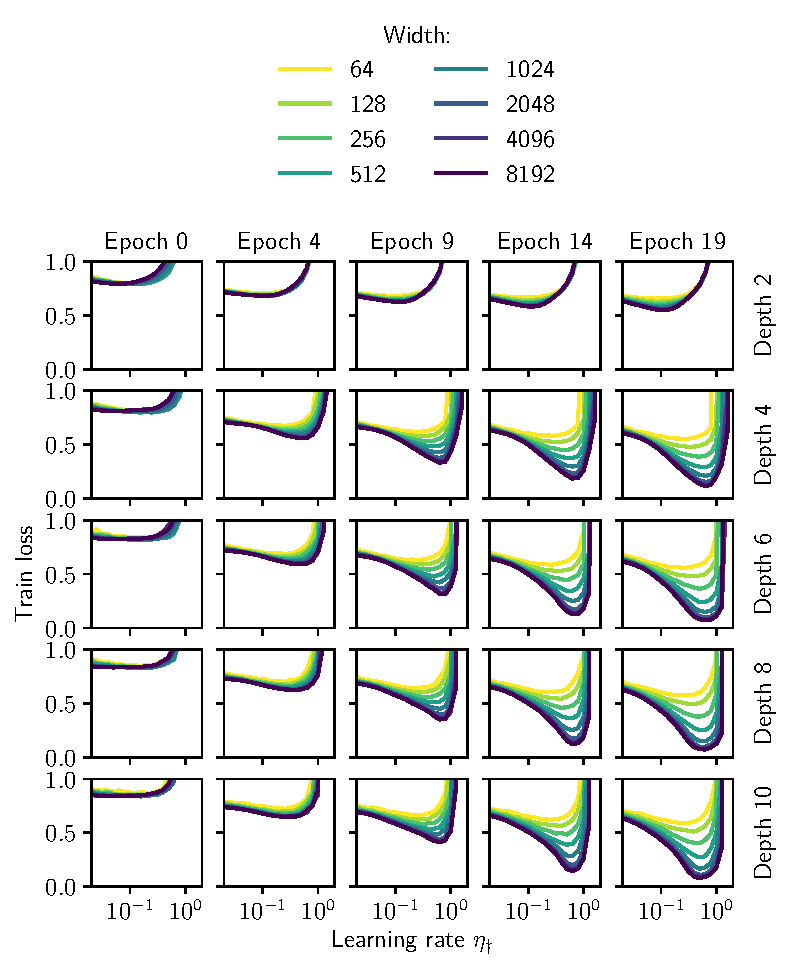
\includegraphics{figures/landscape.pdf}
    \caption[Learning rate transfer across width and depth]{Learning rate transfer across width and depth. Update \ref{eq:opt2} was used to train relu multilayer perceptrons of varying width and depth on the CIFAR-10 dataset. As can be seen, training performance was quite stable as a function of learning rate $\eta_\dagger$, as both width and depth were varied.}
    \label{fig:width-depth}
\end{figure}
\begin{figure}[p]
    \centering
    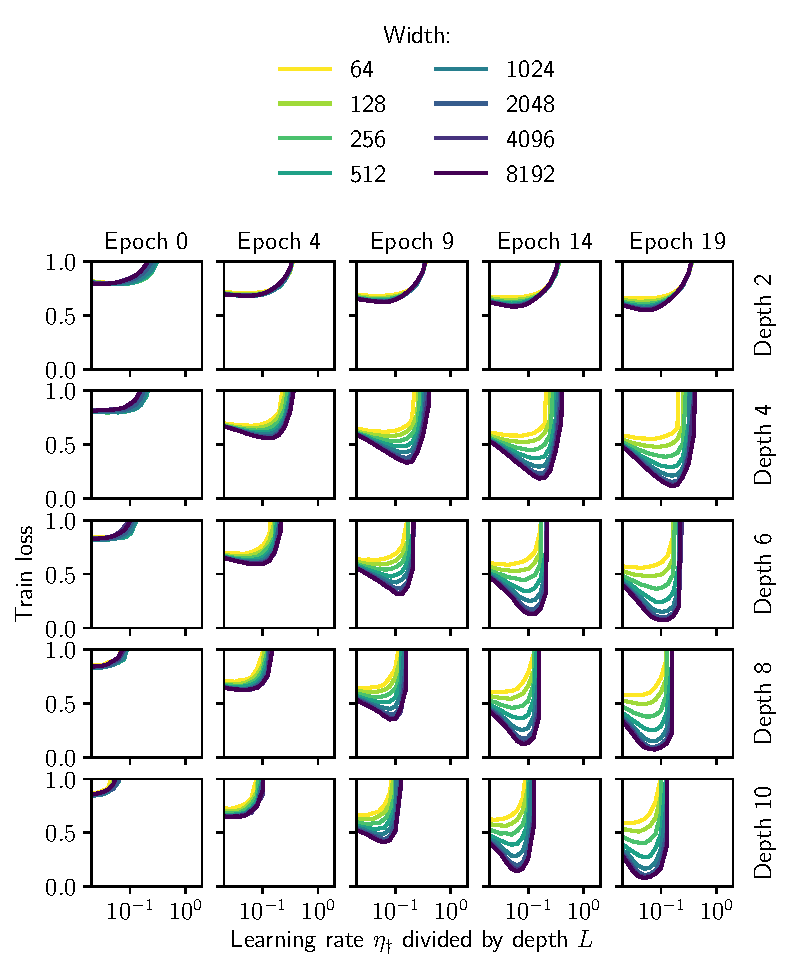
\includegraphics{figures/landscape-lesion.pdf}
    \caption[Learning rate transfer without explicit depth scaling]{Learning rate transfer without explicit depth scaling. The same results as Figure \ref{fig:width-depth} are plotted, except as a function of $\eta_\dagger/L$. This displays the behaviour of Update \ref{eq:opt2} with the explicit depth scaling removed. As can be seen, the tuning curves shift left for increasing depth.}
    \label{fig:width-depth-lesion}
\end{figure}

\clearpage
\printbibliography[heading=subbibliography]
\end{refsection}